%%%%%%%%%%%%%%%%%%%%%%%%%%%%%%%%%%%%%%%%%
% Beamer Presentation
% LaTeX Template
% Version 1.0 (10/11/12)
%
% This template has been downloaded from:
% http://www.LaTeXTemplates.com
%
% License:
% CC BY-NC-SA 3.0 (http://creativecommons.org/licenses/by-nc-sa/3.0/)
%
%%%%%%%%%%%%%%%%%%%%%%%%%%%%%%%%%%%%%%%%%

%----------------------------------------------------------------------------------------
%	PACKAGES AND THEMES
%----------------------------------------------------------------------------------------

\documentclass{beamer}

\mode<presentation> {

% The Beamer class comes with a number of default slide themes
% which change the colors and layouts of slides. Below this is a list
% of all the themes, uncomment each in turn to see what they look like.

%\usetheme{default}
%\usetheme{AnnArbor}
%\usetheme{Antibes}
%\usetheme{Bergen}
%\usetheme{Berkeley}
%\usetheme{Berlin}
%\usetheme{Boadilla}
%\usetheme{CambridgeUS}
%\usetheme{Copenhagen}
%\usetheme{Darmstadt}
%\usetheme{Dresden}
%\usetheme{Frankfurt}
%\usetheme{Goettingen}
%\usetheme{Hannover}
%\usetheme{Ilmenau}
%\usetheme{JuanLesPins}
%\usetheme{Luebeck}
\usetheme{Madrid}
%\usetheme{Malmoe}
%\usetheme{Marburg}
%\usetheme{Montpellier}
%\usetheme{PaloAlto}
%\usetheme{Pittsburgh}
%\usetheme{Rochester}
%\usetheme{Singapore}
%\usetheme{Szeged}
%\usetheme{Warsaw}

% As well as themes, the Beamer class has a number of color themes
% for any slide theme. Uncomment each of these in turn to see how it
% changes the colors of your current slide theme.

%\usecolortheme{albatross}
%\usecolortheme{beaver}
%\usecolortheme{beetle}
%\usecolortheme{crane}
%\usecolortheme{dolphin}
%\usecolortheme{dove}
%\usecolortheme{fly}
%\usecolortheme{lily}
%\usecolortheme{orchid}
%\usecolortheme{rose}
%\usecolortheme{seagull}
%\usecolortheme{seahorse}
%\usecolortheme{whale}
%\usecolortheme{wolverine}

%\setbeamertemplate{footline} % To remove the footer line in all slides uncomment this line
\setbeamertemplate{footline}[page number] % To replace the footer line in all slides with a simple slide count uncomment this line

\setbeamertemplate{navigation symbols}{} % To remove the navigation symbols from the bottom of all slides uncomment this line
}
\usepackage{mathtools}
\usepackage{graphicx} % Allows including images
\usepackage{booktabs} % Allows the use of \toprule, \midrule and \bottomrule in tables
%\usepackage {tikz}
\usepackage[style=ieee]{biblatex}
\usepackage[utf8]{inputenc}
\usepackage[T1]{fontenc}
\usepackage{mathtools}
\usepackage[thinc]{esdiff}
\setbeamertemplate{bibliography item}{\insertbiblabel}
\addbibresource{references.bib}
\title{Bibliography management: \texttt{biblatex} package}
\author{Overleaf}
\date{ }
\DeclareMathOperator*{\argminA}{arg\,min} % Jan Hlavacek
\DeclareMathOperator*{\argminB}{argmin}   % Jan Hlavacek
\DeclareMathOperator*{\argminC}{\arg\min}   % rbp
%\usepackage {xcolor}
\definecolor {processblue}{cmyk}{0.96,0,0,0}
%----------------------------------------------------------------------------------------
%	TITLE PAGE
%----------------------------------------------------------------------------------------

\title[Short title]{Why Does Deep Learning Work?} % The short title appears at the bottom of every slide, the full title is only on the title page

\author{Bhavya Bhatt}
\institute[Indian Institute of Technology Mandi]{
\includegraphics[width=2cm]{Images/logo_hires.jpg}\\Indian Institute of Technology Mandi} % Your institution as it will appear on the bottom of every slide, may be shorthand to save space

\date{July 2020} % Date, can be changed to a custom date

\begin{document}

\begin{frame}
\titlepage % Print the title page as the first slide
\end{frame}

\begin{frame}
\frametitle{Overview} % Table of contents slide, comment this block out to remove it
\tableofcontents % Throughout your presentation, if you choose to use \section{} and \subsection{} commands, these will automatically be printed on this slide as an overview of your presentation
\end{frame}

%----------------------------------------------------------------------------------------
%	PRESENTATION SLIDES
%----------------------------------------------------------------------------------------

%------------------------------------------------


\section{Recap of IB principle}
\begin{frame}{Information Bottleneck Principle}
The central idea of IB-Theory is \footfullcite{IB} \\
\vspace{10mm}
\Large{\centerline{"Regularization by optimal intermediate representations"}}
\end{frame}
\begin{frame}{Mathematical Recapitulation}
    Given $p_{XY}(x, y)$ for the dataset, IB objective is as follows
\[
L(p(\hat{X}|X)) = I(\hat{X}, X) - \beta I(\hat{X}, Y)
\]
and probability distribution of minimum sufficient statistics (optimal) is 
\[
p^{*}(\hat{X}|X)= \argminA_{p(\hat{X}|X)} L(p(\hat{X}|X))
\]
So intermediate representation $\hat{X}$ is a stochastic compressed representation of $X$ 
\end{frame}

\begin{frame}{True optimal and Empirical optimal}
The optimal curve for different $\beta$ with true distribution $p_{XY}(x, y)$ (in black) and with empirical distribution $\hat{p}_{XY}(x, y)$ estimated with finite samples in the dataset is as follows \footnote{Figure taken from \cite{IB}}
\begin{figure}[H]
\centering
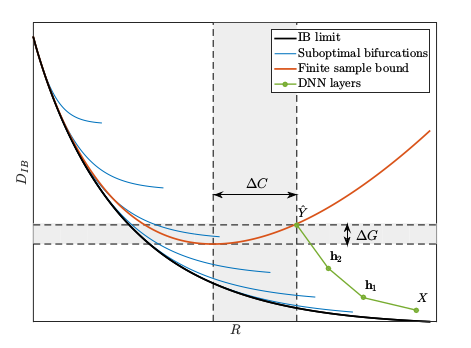
\includegraphics[width=58mm]{Images/IB_curve.png}
\caption{A qualitative information plane, with a hypothesized path of the layers in a typical DNN (green line) on the training data. The black line is the optimal achievable IB limit, and the blue lines are sub-optimal IB bifurcations.}
\end{figure}
\end{frame}

\begin{frame}{Two phase training dynamics - Generalization and Compression phase}
First observed in \cite{BLACKBOXIB}
\begin{figure}[H]
\centering
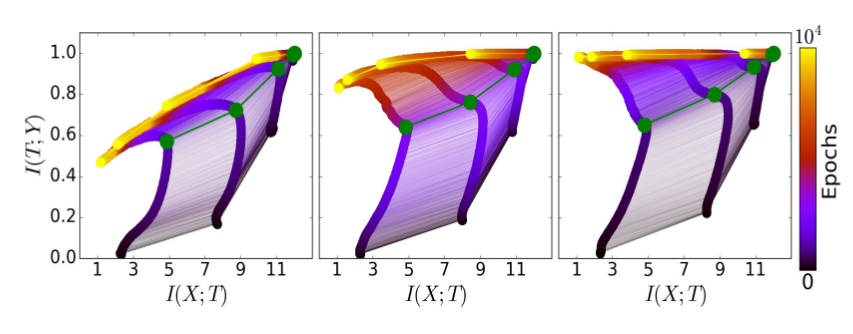
\includegraphics[width=95mm]{Images/two_phase_dynamics.png}
\caption{The evolution of the layers with the training epochs in the information plane. On the left - 5\%, middle - 45\%, and right - 85\% of the data.}
\end{figure}
\footnote{Figure taken from \fullcite{BLACKBOXIB}}
\end{frame}

\begin{frame}{The Controversy}
Paper \cite{ATTACKING} attacked the original paper claiming \footfullcite{ATTACKING}
\vspace{5mm}
\begin{itemize}
        \item IB-Theory is not fundamental theory
        \item Depends on specific activation used
        \item Showed two phase dynamics do not hold for RELU activation
    \end{itemize}
\vspace{5mm}
But later more accurate MI estimators published and observed the two phases ! \\
\vspace{5mm}
Even then , IB-Theory have issues in case of deterministic networks
\end{frame}

\begin{frame}{Resolution - Accurate Mutual Information estimation methods}
Improvement in estimation methods
\vspace{5mm}
\begin{itemize}
        \item Use more accurate MI estimation methods like EDGE, MINE \footnote{MINE - \fullcite{MINE} \\ EDGE - \fullcite{EDGE}}etc.
        \item Use tight bounded MI representations
        \item Research for which estimation method to use when
    \end{itemize}
\end{frame}
\begin{frame}{Problems with Mutual Information}
Problem with mutual information is as follows:
\vspace{5mm}
\begin{itemize}
        \item Difficult to estimate in practice fewer samples available. 
        \item Suffers discontinuity in case of non-stochastic deterministic networks\footfullcite{RANA}.
        \item No measure for robustness to noise.
    \end{itemize}
\end{frame}
\begin{frame}{Dependence Criterion}
Instead of MI as dependence criterion use more robust criterion which captures
\vspace{5mm}
\begin{itemize}
    \item \textbf{inform about $Y$} - $\hat{X}$ should be sufficient statistics
    \item \textbf{be maximally compressed} - representation $\hat{X}$ should not tell about $X$
    \item \textbf{admit a simple decision function} - Y can be estimated from $\hat{X}$ using simple functions
    \item \textbf{be robust} - small noise should not change $\hat{X}$ with big differences
\end{itemize}
\vspace{5mm}
First two are captured by mutual information criterion but there is a need for criterion which captures last two too !
\end{frame}

\begin{frame}{Hilbert Schmidt Independence Criteria}
    An alternate criterion HSIC was first introduced in paper \footfullcite{ma2019hsic}  which gave one of the most interesting application of IB principle \\
    \vspace{10mm}
    \Large{\centerline{"Deep Learning without Back-Propagation"}}
    
\end{frame}

\begin{frame}{PyGlow: Python Package for Information Theory of Deep Learning}
\begin{figure}[H]
\centering

\includegraphics[width=110mm]{Images/PyGlow_complete_logo.jpg}
\end{figure}
\footnote{GitHub repo on: \url{https://github.com/spino17/PyGlow} \\
PyGlow Docs: \url{https://pyglow.github.io/}}
\end{frame}

\section{Information Geometry}
\begin{frame}{Need for Geometric Reformulation}
Need for a geometric framework of information theory:
    \begin{itemize}
        \item Models should not be specified with particular value of parameter\footfullcite{desjardins2015natural}.
        \item Learning dynamics should be independent of parameters.
        \item Distance measure in information theory is non-euclidean.
        \item Coordinate-free formulation to make deep connections of information theory with DL visible.
    \end{itemize}
\end{frame}

\begin{frame}{Ingredients - Manifolds}
    Manifolds - Topological spaces which locally looks like $\mathbb{R}^{n}$.
    \begin{figure}
        \centering
        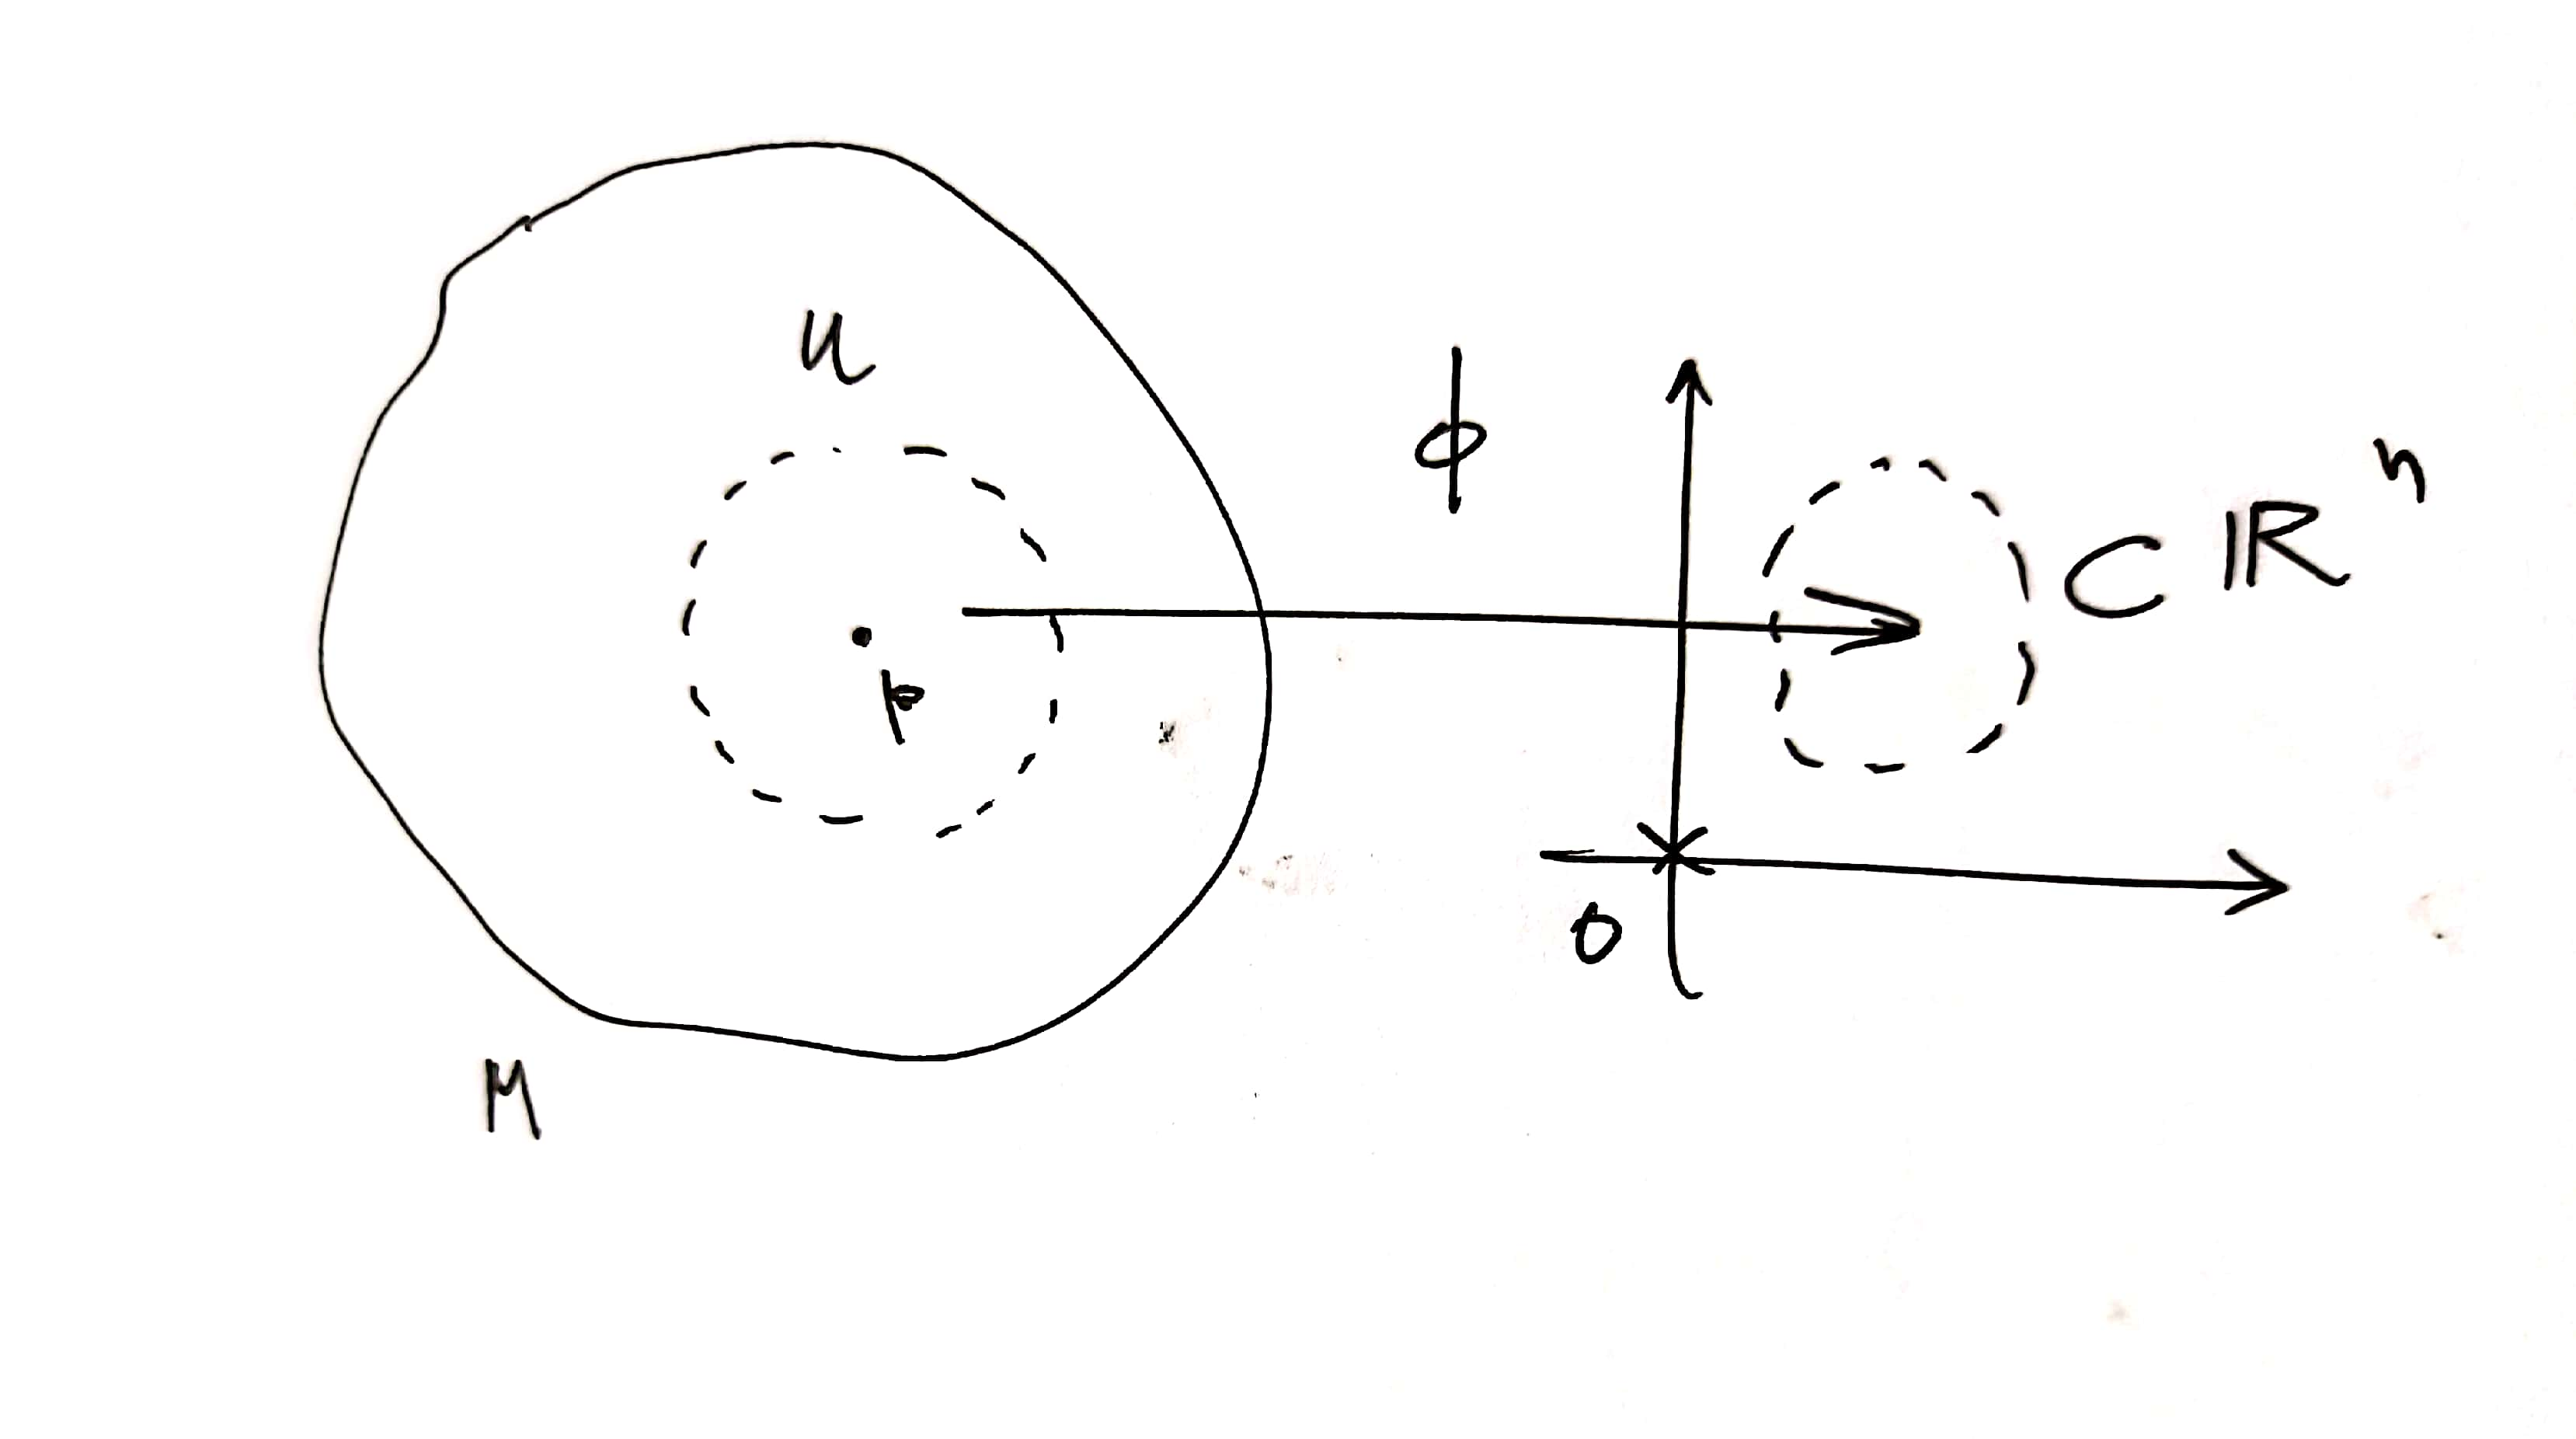
\includegraphics[scale=0.08]{Images/image_6.jpeg}
        \label{fig:fig_1}
    \end{figure}
    For any point $p\in M$, there exists an open set $U$ such that we have a homeomorphism from $U$ to $\mathbb{R}^{n}$.
\end{frame}
\begin{frame}{Ingredients - Vectors}
    Vectors - Objects that captures the rate with which a function $f\colon M\to \mathbb{R}$ on manifold changes along a curve $\gamma\colon [0, 1]\to M$. They live in tangent space $T_{p}M$.
    \begin{equation*}
        V_{\gamma}[f] = \diff{f\circ\gamma(\lambda)}{\lambda}\Bigr|_{\lambda = 0}
    \end{equation*}
    \begin{figure}
        \centering
        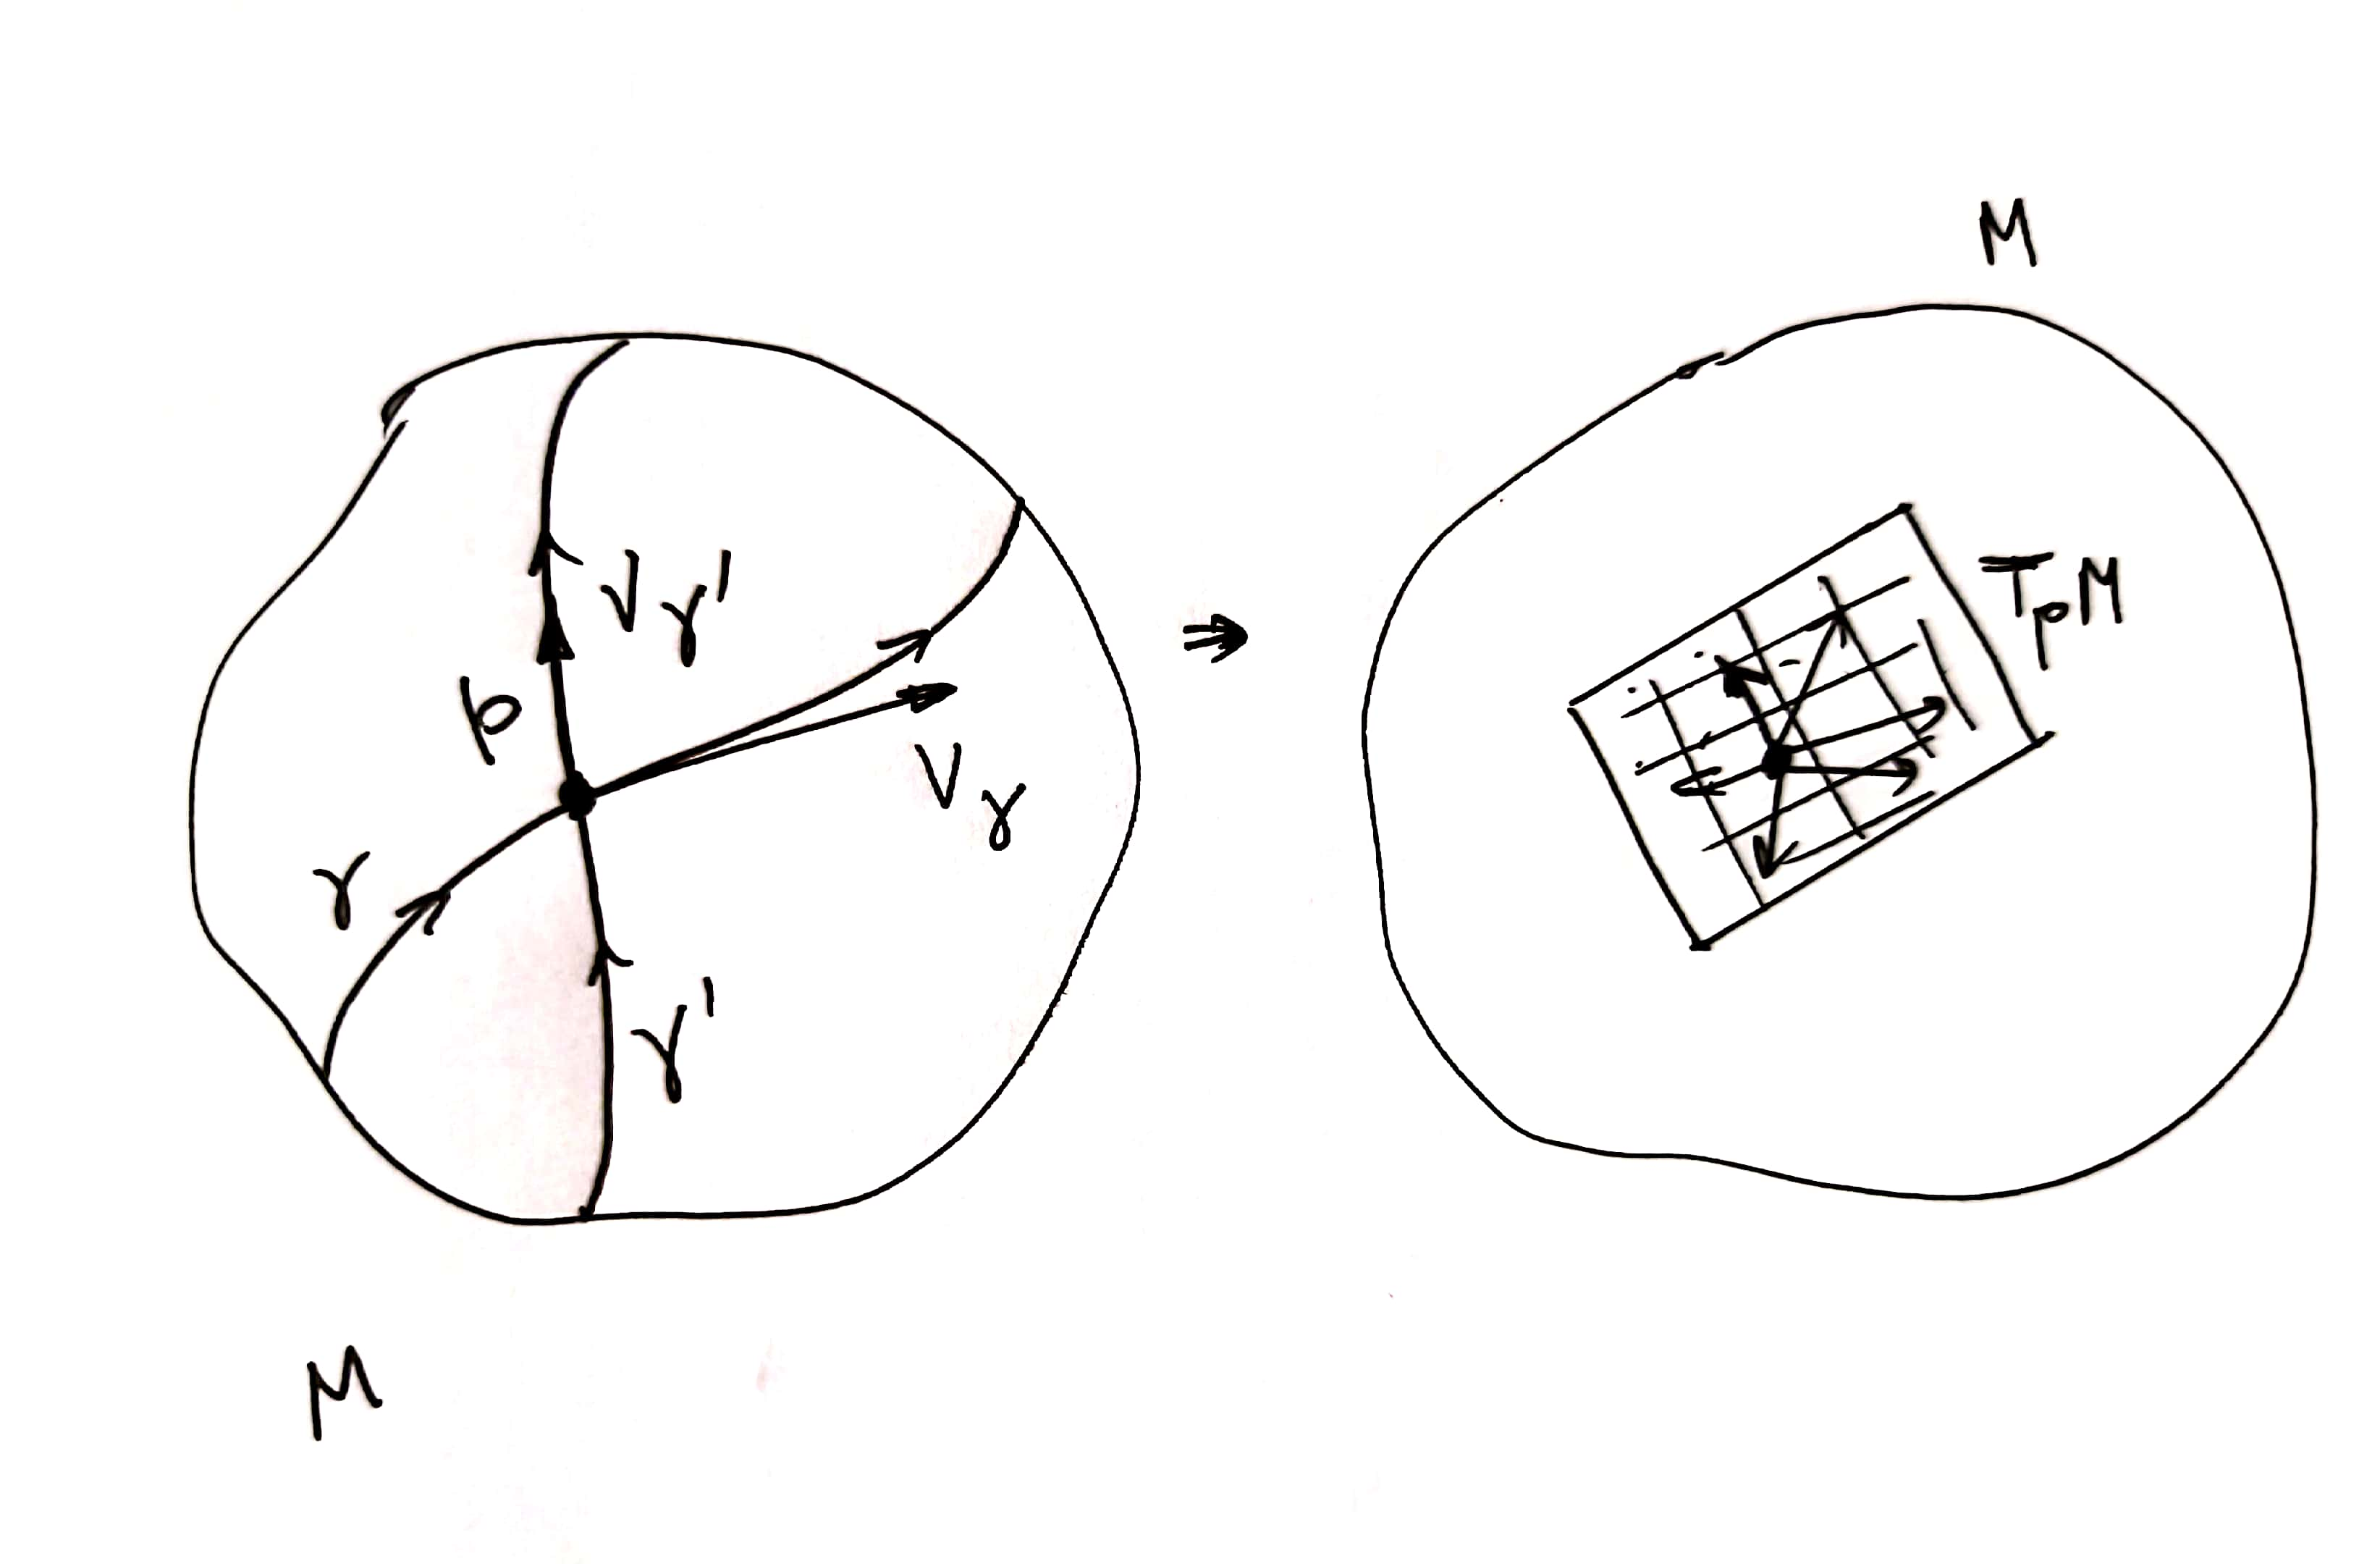
\includegraphics[scale=0.06]{Images/image_8.jpeg}
        \label{fig:fig_2}
    \end{figure}
    Basis of $T_{P}M$ - $\{\partial_{\alpha} = \frac{\partial}{\partial x ^{\alpha}}\Bigr|_{p}\}_{\alpha = 1\dots n}$
\end{frame}
\begin{frame}{Ingredients - One-forms}
    One-forms - Objects that take vectors from abstract objects to a point in $\mathbb{R}^{n}$ (components of vectors in common treatments). They live in cotangent dual space $T^{\ast}_{p}M$.
    \begin{equation*}
         df(V) \coloneqq V[f]\in \mathbb{R}
    \end{equation*}
    This object is called as gradient of a function $f$. We now define dual basis $\omega_{\alpha}$ of $T^{\ast}_{p}M$, which are dual to the coordinate basis of $T_{p}M$ as
    \begin{equation*}
        \omega_{\alpha}(\frac{\partial}{\partial x^{\beta}}\Bigr|_{p}) \coloneqq \delta^{\alpha}_{\beta}
    \end{equation*}
    Basis of $T^{\ast}_{p}M$ - $\{dx^{\alpha}\}_{\alpha=1\dots n}$
\end{frame}
\begin{frame}{Ingredients - Metric Tensor}
    Metric Tensor - Gives a notion of length (via infinitesimal lengths) on the manifold.
    $g_{p}\colon T_{p}M \times T_{p}M\to \mathbb{R}$ as
    \begin{equation*}
        g_{p}(U, V) = \langle U, V\rangle
    \end{equation*} for any $U, V\in T_{p}M$.
    In coordinate basis,
    \begin{equation*} 
        g = g_{\alpha\beta}(p)dx^{\alpha}\otimes dx^{\beta}
    \end{equation*}
    for example: $ds^{2} = dr^{2} + r^{2}d\theta^{2} + r^{2}\sin^{2}\theta d\phi^{2}$ is infinitesimal length on sphere in spherical coordinates basis.
\end{frame} 
\begin{frame}{Ingredients - Affine Connections}
    Affine Connection - Provides us with a definition of parallel transport and directional derivative.
    \begin{figure}
       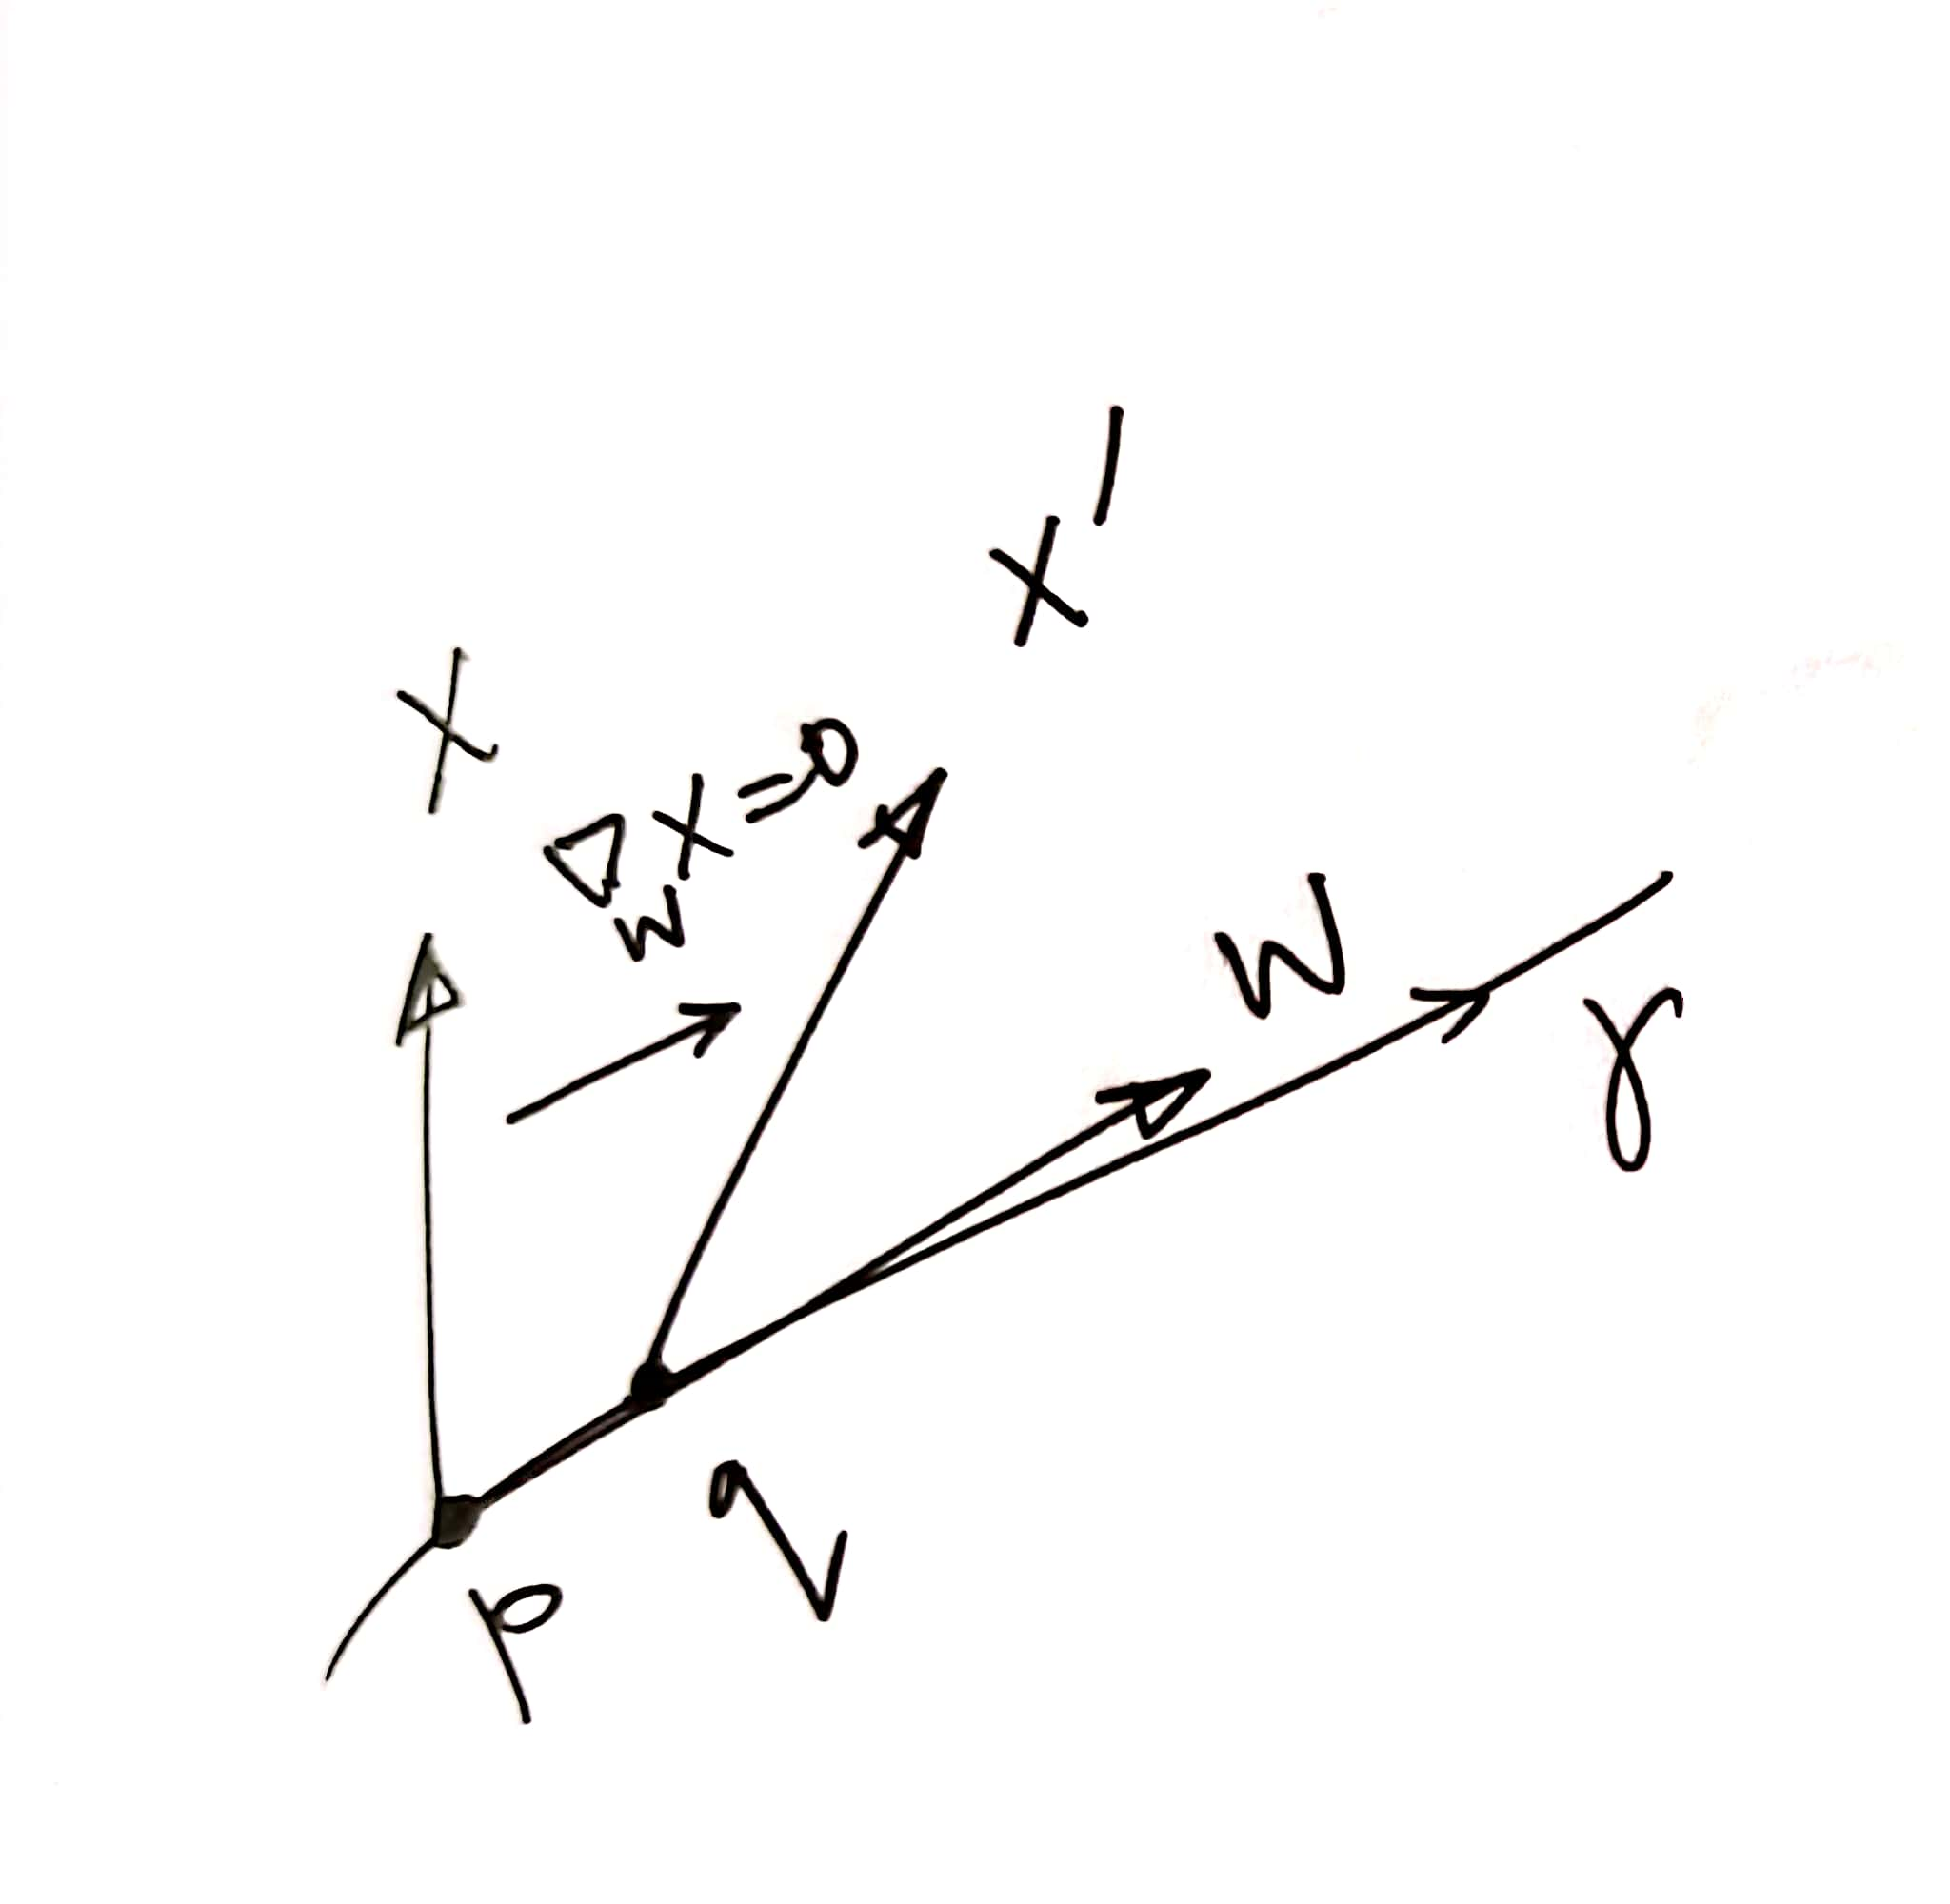
\includegraphics[scale=0.06]{Images/image_9.jpeg}
       \label{fig:fig_3}
    \end{figure}
    For a vector $X\in T_{p}M$, the parallel transport vector $X^{\prime}\in T_{q}M$ along the curve $\gamma$ with tangent vector $W$ is 
    \begin{equation*} 
        X^{\prime\alpha}(q) = X^{\alpha}(p) - \Gamma^{\alpha}_{\beta\gamma}(p)W^{\gamma}X^{\beta}\Delta \lambda
    \end{equation*} where $\Gamma^{\alpha}_{\beta\gamma}$ are christoffel symbols which captures curvi-linearity of coordinate systems.
\end{frame}
\begin{frame}{Affine Connections}
    The covariant derivative $\nabla_{W}X$ w.r.t to connection $\nabla$ is given by
    \begin{equation*}
        \nabla_{W}X = \diff{X^{\alpha}}{\lambda} + \Gamma^{\alpha}_{\beta\gamma}W^{\gamma}X^{\beta}
    \end{equation*}
    Metric Induced Connection:
    \begin{itemize}
        \item Metric compatibility - X[g(Y, Z)] = 0 for $Y, Z$ being parallel transported along $X$.
        \item Torsion Free - $\Gamma^{\alpha}_{\beta\gamma} = \Gamma^{\alpha}_{\gamma\beta}$. 
    \end{itemize} These restriction are enough to obtain closed form expression for christoffel symbols 
    \begin{equation*}
        ^{LC}\Gamma^{\alpha}_{\beta\gamma} = \frac{1}{2}g^{\alpha\lambda}(\partial_{\gamma}g_{\lambda\beta} + \partial_{\beta}g_{\gamma\lambda} -\partial_{\lambda}g_{\beta\gamma})
    \end{equation*} where $^{LC}\Gamma^{\alpha}_{\beta\gamma}$ is Levi-Civita christoffel symbols. \\
    \vspace{5mm}
    Fundamental Theorem of Riemannian Geometry - The above Levi-Civita connections are unique.
\end{frame}
\begin{frame}{Information Manifolds - (M, g, $\nabla$, $\nabla^{\ast}$)}
    Conjugate-Connection Manifolds - Spaces of allowed parameters for a statistical decision making problem. The CCM's have a dual structure of connections $(\nabla, \nabla^{\ast})$ with $\nabla^{\ast}$ defined by:
    \begin{equation*}
        X[g(Y,Z)] = g(\nabla_{X} Y, Z) + g(Y, \nabla^{\star}_{X} Z)
    \end{equation*} for any arbitrary vector fields $X, Y$ and $Z$. \\
    \vspace{5mm}
    Note: $(\nabla^{\star})^{\star} = \nabla$.
    Equivalent definition - 
    \begin{equation*}
        \langle U, V\rangle = \langle \prod^{\nabla}_{\gamma(t)}U, \prod^{\nabla^{\star}}_{\gamma(t)}V\rangle
    \end{equation*} which is statement that dual connections are metric-preserving. Note from this definition Levi-Civita Connection is self-dual $(^{LC}\nabla, ^{LC}\nabla^{\ast} = ^{LC}\nabla)$
\end{frame}
\begin{frame}{Statistical Manifolds}
    A statistical manifold $(M, g, C)$ is a manifold equipped with a metric tensor $g$ and a totally symmetric 3-tensor $C$ Amari-Chentsov tensor where
    \begin{equation*}
        C(X, Y, Z) \coloneqq \langle\nabla_{X}Y - \nabla^{\star}_{X}Y, Z\rangle
    \end{equation*} or in component form
    \begin{equation*}
        C^{k}_{ij} = \Gamma^{k}_{ij} - \tilde{\Gamma}^{k}_{ij}
    \end{equation*} Also for given pair $(\Gamma^{\alpha}_{\beta\gamma}, \tilde{\Gamma}^{\alpha}_{\beta\gamma})$, we have a self-dual connection 
    \begin{equation*}
        ^{LC}{\nabla} = \frac{1}{2}(\nabla + \nabla^{\star})
    \end{equation*} which from fundamental theorem of Riemannian Geometry is Levi-Civita connections.
\end{frame}
\begin{frame}{One-parameter family of Conjugate Connections}
    For a given $(\Gamma^{\alpha}_{\beta\gamma}, \tilde{\Gamma}^{\alpha}_{\beta\gamma})$ with Amari-Chentsov tensor $C^{\alpha}_{\beta\gamma}$. \\
    \vspace{5mm}
    Then for a continous parameter $\lambda$, $\lambda C^{\alpha}_{\beta\gamma}$ is also totally symmetric tensor and can be Amari-Chentsov tensor of some other pair of dual connections $(\nabla^{-\lambda}, (\nabla^{-\lambda})^{\ast} = \nabla^{\lambda})$ with christoffel symbols as:
    \begin{align*}
       \Gamma^{\lambda}_{ijk} = \Gamma^{0}_{ijk} - \frac{\lambda}{2}C_{ijk} \\
       \Gamma^{-\lambda}_{ijk} = \Gamma^{0}_{ijk} + \frac{\lambda}{2}C_{ijk}
\end{align*} where $\Gamma^{0}_{ijk}$ is Levi-Civita connections. \\
\vspace{5mm}
Fundamental Theorem of Information Geometry - A manifold $(M, g, \nabla^{-\lambda}, \nabla^{\lambda})$ is $\nabla^{\lambda}$-flat if and only if it is $\nabla^{-\lambda}$-flat.
\end{frame}
\begin{frame}{Big Question - How can we obtain above structures ?}
    Two ways to obtain CCM structure $(g, \nabla, \nabla^{\ast})$ canonically from the problem is:
    \begin{itemize}
        \item From divergence considered in the problem to capture dissimilarity between probability distributions.
        \item From probability distribution itself by using max-log likelihood principle.
    \end{itemize}
    \vspace{10mm}
\end{frame}
\begin{frame}{Conjugate Connection Structure from Divergences}
Divergence: \\
$D\colon M \times M \to [0, \infty)$ on a manifold $M$ with a local chart $\theta \subset \mathbb{R}^{D}$ with following properties
\begin{itemize}
    \item $D(\theta:\theta^{\prime})$ $\geq 0$ $\forall$ $\theta, \theta^{\prime} \in \Theta$ where equality holds if and only if $\theta = \theta^{\prime}$.
    \item $\partial_{i, .}D(\theta, \theta^{\prime})\Bigr|_{\theta=\theta^{\prime}} = \partial_{., j}D(\theta, \theta^{\prime}\Bigr|_{\theta=\theta^{\prime}} = 0$ $\forall i, j$ 
    \item $-\partial_{., i}\partial_{., j}D(\theta, \theta^{\prime})\Bigr|_{\theta=\theta^{\prime}}$ is positive-definite.
\end{itemize}We can also define a dual-divergence by swapping the arguments
\begin{equation*}
    D^{\star}(\theta, \theta^{\prime}) = D(\theta, \theta^{\prime})
\end{equation*}
Intuition: 
    \begin{align*}
        D(\theta, \theta + \delta\theta) &= D(\theta, \theta) + \frac{\partial}{\partial \theta^{i}}D\Bigr|_{\theta}\delta\theta + \frac{\partial^{2}}{\partial\theta^{i}\partial\theta^{j}}D\Bigr|_{\theta}\delta\theta^{i}\delta\theta^{j} \\
                                     &= \frac{\partial^{2}}{\partial\theta^{i}\partial\theta^{j}}D\Bigr|_{\theta}\delta\theta^{i}\delta\theta^{j} \\
                                     &= \partial_{i, j}D(\theta, \theta^{\prime})\Bigr|_{\theta}\delta\theta^{i}\delta\theta^{j}
    \end{align*}
\end{frame}
\begin{frame}{Conjugate Connection Structure from Divergences}
    we define the conjugate connection structure naturally induced by divergence $D(\theta, \theta^{\prime})$ as follows:
\begin{itemize}
    \item $g\coloneqq -\partial_{i, j}D(\theta, \theta^{\prime})\Bigr|_{\theta=\theta^{\prime}}$
    \item $\Gamma_{ijk}\coloneqq -\partial_{ij, k}D(\theta, \theta^{\prime})\Bigr|_{\theta=\theta^{\prime}}$
    \item $\tilde{\Gamma}_{ijk}\coloneqq -\partial_{k, ij}D(\theta, \theta^{\prime})\Bigr|_{\theta=\theta^{\prime}}$
\end{itemize}
\end{frame}
\begin{frame}{Conjugate Connection Structure from Probability Distribution}
    Let $\mathfrak{P}$ be a parametric family of probability distribution
\begin{equation*}
    \mathfrak{P}=\{p_{\theta}(X)\}_{\theta\in \Theta}
\end{equation*} where $\Theta$ is parameter space. Order of parameter space is dimension of parameter space. We use the familiar log-likelihood function
\begin{equation*}
    l(\theta; x) = \log p_{\theta}(x) 
\end{equation*}
We now define metric as 
\begin{equation*}
    I(\theta) = g_{ij} = \mathbb{E}_{\theta}[\partial_{i}l\partial_{j}l]
\end{equation*}
This relates with the Cramer-Rao lower bound on variance of estimator
\begin{equation*}
    Var_{\theta}[\hat{\theta}_{n}(x)] \geq \frac{1}{n}I^{-1}(\theta)
\end{equation*}
\end{frame}
\begin{frame}{Conjugate Connection Structure from Probability Distribution}
    Now we define two types of connections which is naturally defined in terms of the above probability distribution
    \vspace{10mm}
\begin{itemize}
    \item Exponential connection - $^{e}\Gamma_{ijk} \coloneqq \mathbb{E}_{\theta}[(\partial_{i}\partial_{j}l)\partial_{k}l]$
    \vspace{5mm}
    \item Mixing connection - $^{m}\Gamma_{ijk} \coloneqq \mathbb{E}_{\theta}[(\partial_{i}\partial_{j}l + \partial_{i}l\partial_{j}l)\partial_{k}l]$
\end{itemize}
\vspace{5mm}
For a complete treatment on the subject refer  the paper \footfullcite{nielsen2018elementary}.
\end{frame}
\begin{frame}{Why this is relevant in Deep Learning?}
    Natural Gradient Descent - If the problem has non-euclidean information manifold (which is the case most of the time) then the update rule in gradient descent algorithm is given by
    \begin{equation*}
        \theta_{t+1} = \theta_{t} - \eta_{t}\tilde{\nabla}l(\theta)
    \end{equation*} Here $\tilde{\nabla}$ is natural gradient defined as\footfullcite{amari}
    \begin{equation*}
        \tilde{\nabla}l(\theta) = G^{-1}\nabla l(\theta)
    \end{equation*} where $\nabla = (\frac{\partial}{\partial x^{1}}, \dots, \frac{\partial}{\partial x^{n}})$ is usual gradient and $G = g_{\alpha\beta}$.
\end{frame}
\section{Future Work}
 \begin{frame}{Scope of Future Work - Classical VS Non-Classical Models}
    Classical Probability - Source of stochastic outcome comes from the missing of intractable hidden variables from the dynamics. For example: tossing of coin\footnote{Image Source - https://www.bellevuerarecoins.com/history-coin-flip/}
    \begin{figure}
        \centering
        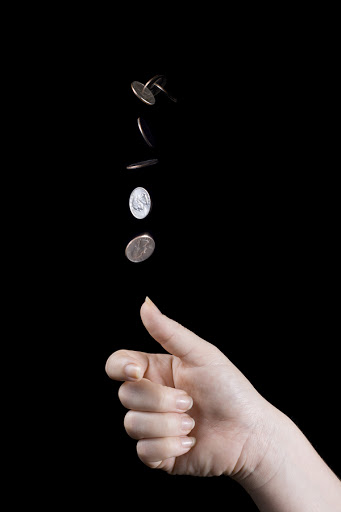
\includegraphics[scale=0.2]{Images/unnamed.jpg}
        \label{fig:fig_4}
    \end{figure}
    Non-classical Probability - Stochastic outcomes are intrinsic even if the dynamics is complete (no local hidden variables missing). For example: quantum probability
 \end{frame}
 \begin{frame}{Scope of Future Work - Bell's Inequality}
     How to distinguish between classical and non-classical probabilities? \\
     \vspace{10mm}
     \Large{\centerline{"Bell's Inequality"}}
     \vspace{10mm}
     
     Classical Probability - Obeys Bell's Inequality. \\
     \vspace{5mm}
     Non-Classical Probability - Does not obey Bell's inequality.
     \footfullcite{Bell2004-BELOTE}
 \end{frame}
 \begin{frame}{Scope of Future Work - Classical VS Non-Classical Models}
     Two main features of dynamical theories which obey Bell's Inequality:
     \begin{itemize}
         \item Counter-factual definiteness.
         \item Local hidden variables.
     \end{itemize}
     \begin{figure}
         \centering
         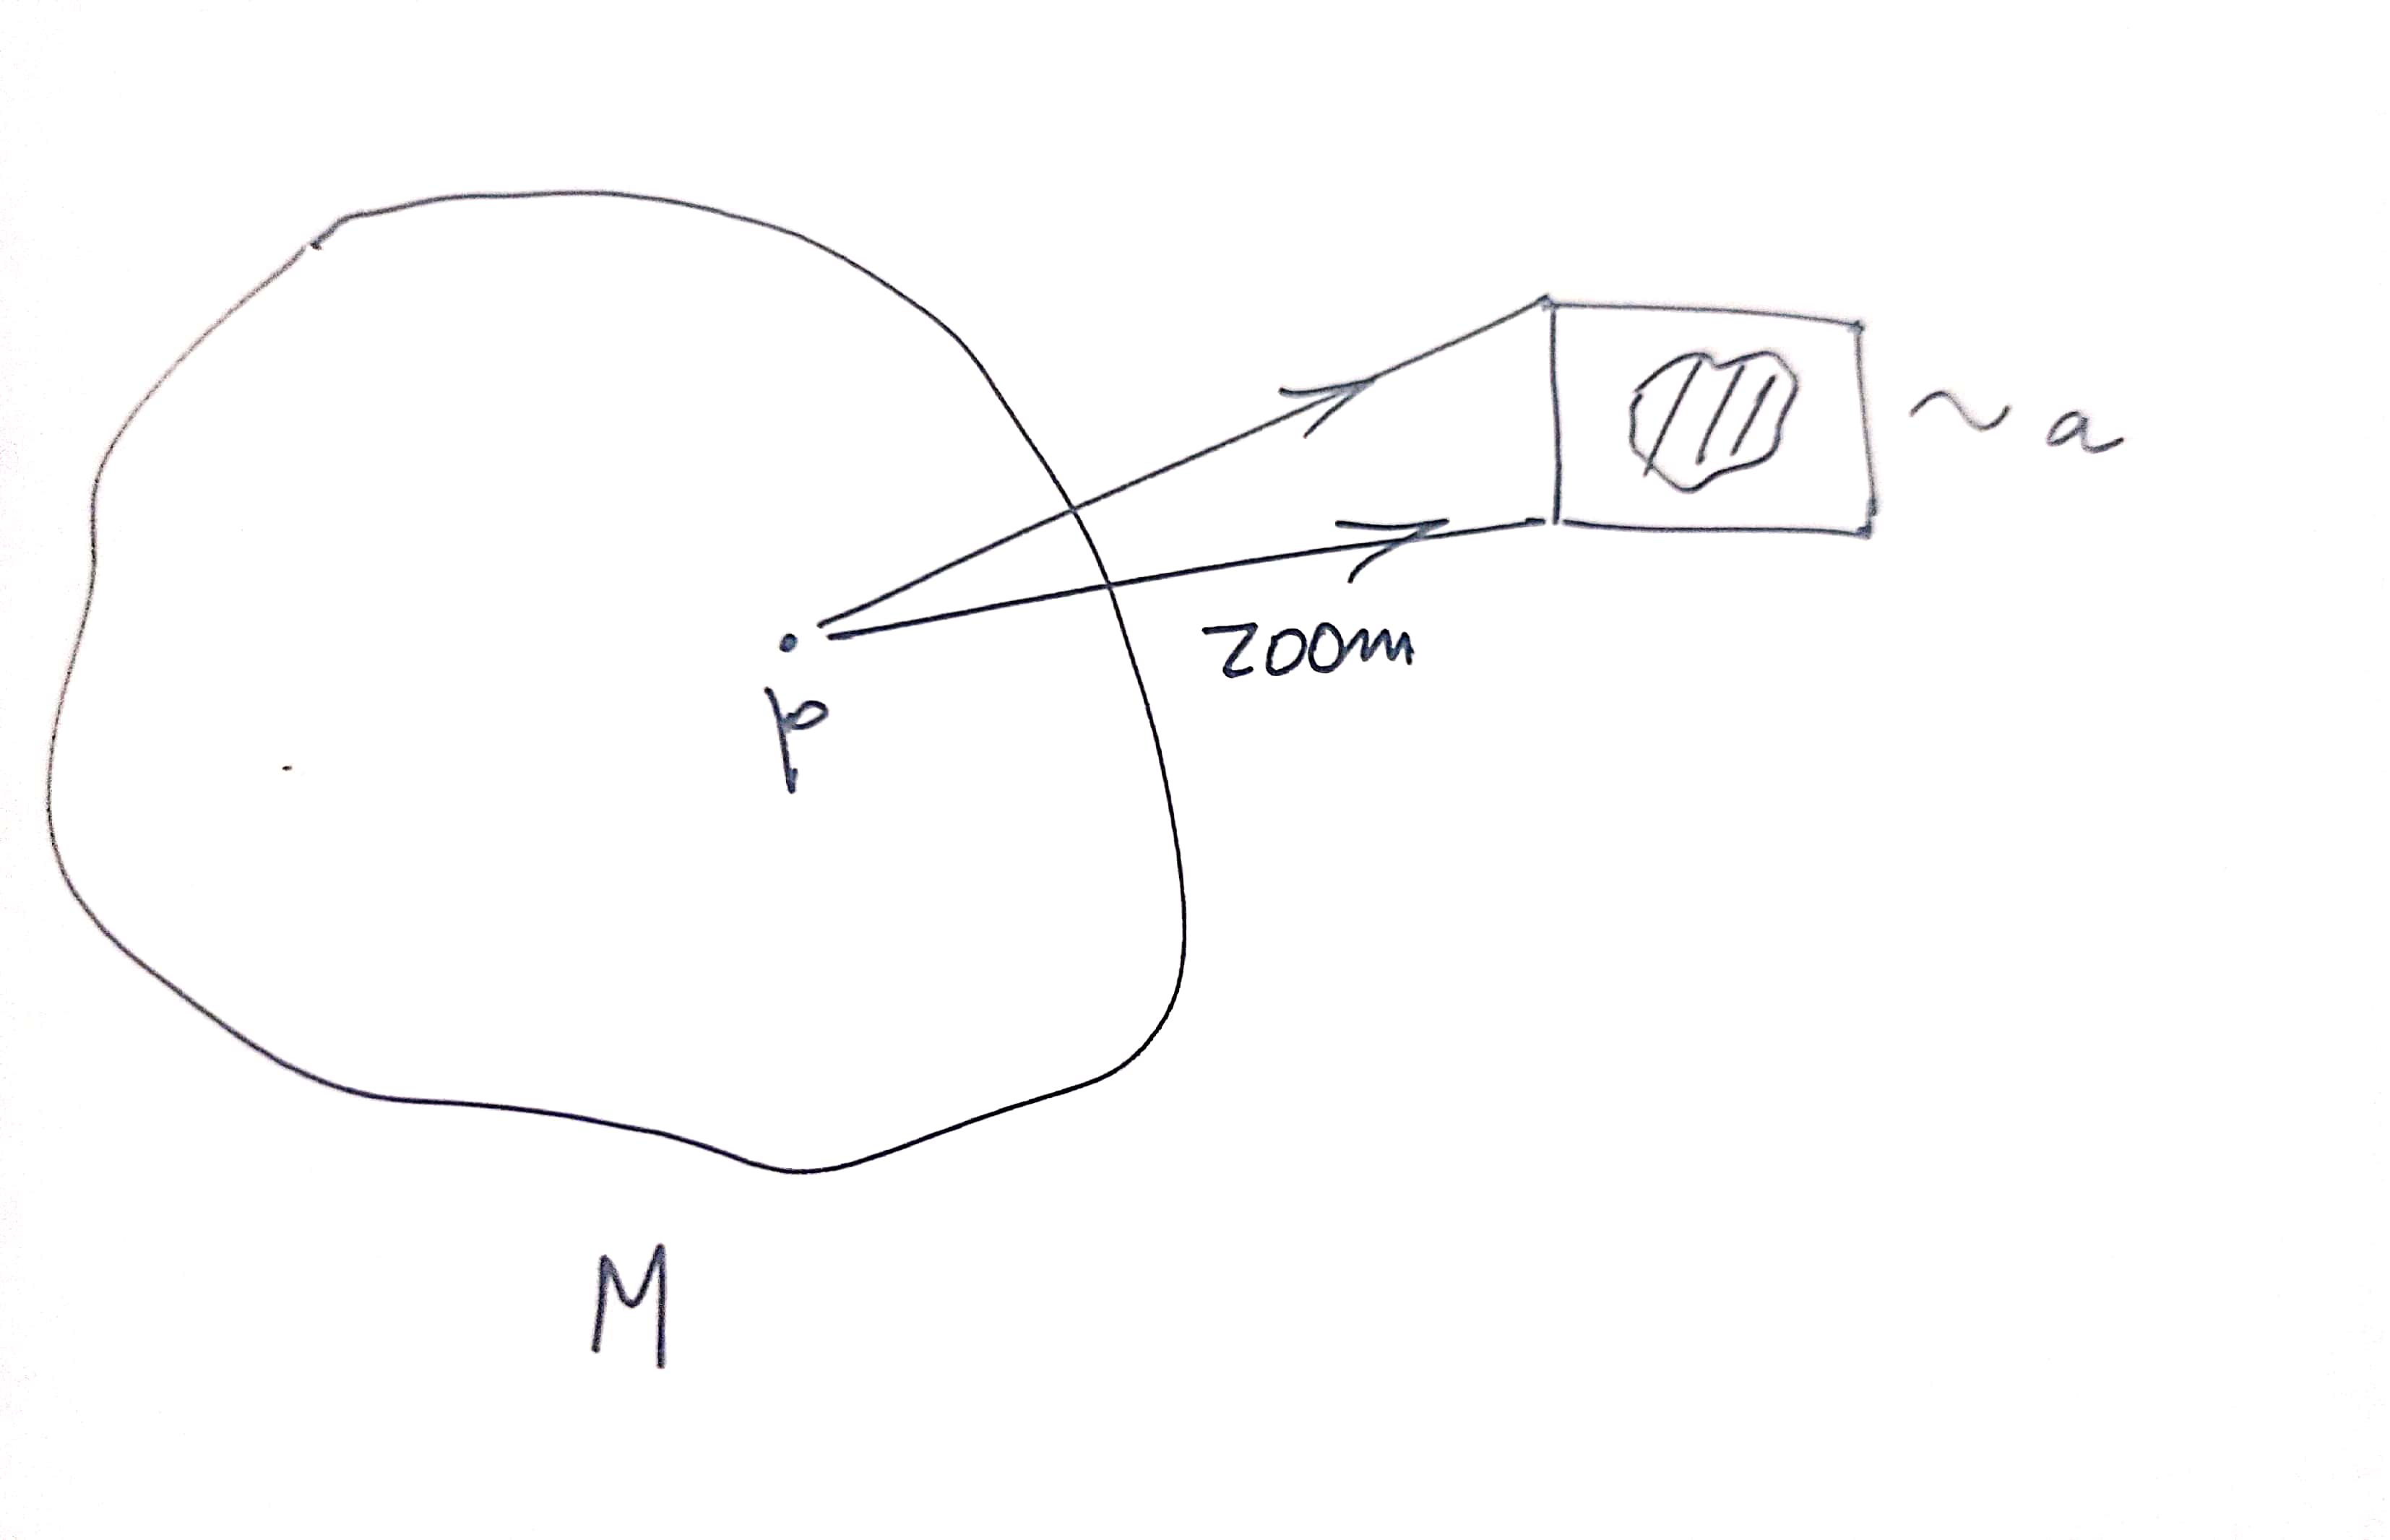
\includegraphics[scale=0.07]{Images/image_10.jpeg}
         \label{fig:fig_5}
     \end{figure}
     In this diagram above, $a$ is the order of intrinsic uncertainty. For quantum mechanics $a$ is $\hbar$. 
 \end{frame}
 \begin{frame}{Scope of Future Work - Classical VS Non-Classical Models}
     Classical information manifolds are non-classical information manifolds in the limit $a\longrightarrow 0$. \\
     For reverse, from classical information manifolds to non-classical information manifolds, the process is called \\
     \vspace{10mm}
     \Large{\centerline{"Quantization"}}
     \vspace{10mm}
     Quantization: real chart coordinates $\theta_{\alpha} \in \mathbb{R}\longrightarrow$ matrix-valued operators $\Theta_{\alpha}$ (finite or infinite dimensional)
     \begin{equation*}
         [\Theta_{\alpha}, \Theta_{\beta}] \sim a\Delta_{\alpha\beta}\mathbb{I}
     \end{equation*} where $\Delta_{\alpha\beta}$ quantifies uncertainty coefficient between different pairs $(\alpha, \beta)$.
 \end{frame}
 \begin{frame}{Scope of Future Work - Are Deep Neural Networks non-classical?}
     Do hidden layers have non-classical stochastic nature ? \\
     \vspace{10mm}
     \Large{\centerline{"Analyse Classical Information Manifolds for DNN"}}
     \vspace{10mm}
 \end{frame}
\begin{frame}
\Huge{\centerline{Thank You}}
\end{frame}

%------------------------------------------------

\begin{frame}[allowframebreaks]
\frametitle{References}
\printbibliography

\end{frame}
%----------------------------------------------------------------------------------------
\end{document}